
% Morten -- jeg skriver bare en veldig plain tex-fil her, så kan du gjøre det du vil med innholdet etterpå.


\documentclass{article}
\usepackage[utf8]{inputenc}
\usepackage[a4paper]{geometry}
\usepackage[norsk]{babel}
\usepackage{amssymb}
\usepackage{amsmath}
\usepackage{amsthm}
\usepackage{multicol}
\usepackage{scrextend}
\usepackage{mdframed}
\usepackage{hyperref}
\usepackage{listings}
\usepackage{tikz}
\usetikzlibrary{patterns,decorations.pathmorphing, decorations.pathreplacing}
\usepackage{pgfplots}
\usepackage{array}
\usepackage{mdframed}
\usepackage[american]{circuitikz}
\usepackage[small]{titlesec}

\hypersetup{colorlinks=true, 
    linkcolor=blue, 
    filecolor=magneta,
    urlcolor=cyan,
    citecolor=black,
}

\setlength{\parindent}{0em}
\setlength{\parskip}{1em}

\theoremstyle{plain}
\newtheorem{thm}{Teorem}\surroundwithmdframed{thm}
\newtheorem{prop}[thm]{Proposisjon}

\theoremstyle{definition}
\newtheorem{defnx}[thm]{Definisjon}
\newtheorem{exx}[thm]{Eksempel}
\newtheorem{bevisskisse}[thm]{Skisse av bevis}

\theoremstyle{remark}
\newtheorem{remarkx}[thm]{Merknad}

\newenvironment{defn}
{\pushQED{\qed}\renewcommand{\qedsymbol}{$\triangle$}\defnx}
{\popQED\enddefnx}
\newenvironment{ex}
{\pushQED{\qed}\renewcommand{\qedsymbol}{$\triangle$}\exx}
{\popQED\endexx}
\newenvironment{remark}
{\pushQED{\qed}\renewcommand{\qedsymbol}{$\triangle$}\remarkx}
{\popQED\endremarkx}


% Endre på disse etter hvilken notasjon du vil ha.
\newcommand{\diff}[1]{\mathop{d#1}} 
\newcommand{\fcn}{x}
\newcommand{\boldvec}[1]{\boldsymbol{\mathrm{#1}}}
\newcommand{\expfcn}[1]{e^{#1}}
\newcommand{\abs}[1]{|#1|}
\newcommand{\bigabs}[1]{\big|#1\big|}
\newcommand{\biggabs}[1]{\bigg|#1\bigg|}
\newcommand{\bigparanth}[1]{\big(#1\big)}
\newcommand{\biggparanth}[1]{\bigg(#1\bigg)}
\newcommand{\bigbrac}[1]{\big[#1\big]}
\newcommand{\biggbrac}[1]{\bigg[#1\bigg]}
\newcommand{\imagunit}{\mathrm{j}}

\DeclareMathOperator{\imaginary}{Im}
\DeclareMathOperator{\real}{Re}


\title{Førsteordens differensialligninger}
\author{}
\date{}

\begin{document}
\maketitle

Dette kapitlet er en introduksjon til førsteordens ordinære differensialligninger. Vi skal se på både lineære og ikkelineære ligninger. For lineære differensialligninger finnes det god teori på eksistens og unikhet av løsninger, flere universelle løsningsteknikker, og vi kan ofte finne analytiske løsninger for disse. Dette gjelder i mye mindre grad for ikkelineære ligninger. For disse er det mye vanskeligere å utlede analytiske løsninger, og vi er avhengig av kvalitative eller numeriske metoder.

Vi begynner med å se på noen eksempler hvor differensialligninger oppstår som modeller for fysiske situasjoner. Vi skal komme tilbake til hvordan vi kan løse disse mot slutten av dette notatet.

\begin{ex} \label{eks:krets_1}
    Følgende figur viser en (RL-)krets med en spenningskilde, en motstand og en spole.
    \begin{center}
        \begin{circuitikz}
            \draw
            (0,0)
            to[american voltage source, voltage dir=old, l={$V_s$}, i^={$I(t)$}] (0,3)
            to[european resistor, l_ = $R$] (3,3)
            to (3,0)
            to[cute inductor, l_ = $L$] (0, 0);
        \end{circuitikz}
    \end{center}
    Ved Ohms lov er spenningsfallet over motstanden lik $RI$ og spenningsfallet over spolen er $L\dot{I}$. Kirchhoffs spenningslov, som sier at summen av potensialforskjellene over en lukket strømsløyfe må utligne hverandre, gir dermed at
    \begin{equation*}
        \dot{I} + \frac{R}{L} I = \frac{V_s}{L}.
    \end{equation*}
    Dette er et eksempel på en førsteordens lineær differensialligning, hvor den ukjente er funksjonen $I(t)$.
\end{ex}

\begin{ex} \label{eks:newtons_kj_lov_1}
    Newtons kjølelov sier at endringen i temperaturen til et objekt er direkte proporsjonal med temperaturforskjellen mellom objektet og omgivelsene. Dersom Sindre skal steke ribbe til julaften kan temperaturen til ribben etter at det er satt inn i ovnen bestemmes ved å løse
    \begin{equation*}
        \dot{T} = k(T - T_0).
    \end{equation*}
    Proporsjonalitetskonstanten $k$ for systemet må riktignok bestemmes først, men dette kan Sindre selv gjøre på en eller annen måte.
\end{ex}

\begin{ex} \label{eks:populasjon_1}
    I studet av populasjonsvekst møter man ofte den logistiske ligningen
    \begin{equation*}
        \dot{\fcn}(t) = A \fcn(t) - B (\fcn(t))^2,
    \end{equation*}
    hvor $\fcn(t)$ beskriver en populasjonsstørrelse som funksjon av tid. Dersom vi setter $B = 0$ får vi en malthusiansk modell, etter den britiske samfunnsøkonomen Thomas Robert Malthus, som gir eksponensiell populasjonsvekst. Senere skal vi se at leddet $-B \fcn^2$ begrenser veksten i populasjonsmodellen.
\end{ex}


\section*{En kort oversikt}

En førsteordens differensialligning er en relasjon mellom en funksjon og dens deriverte. Vi skal her jobbe utelukkende med ordinære differensialligninger, altså ligninger for funksjoner med bare én ukjent. Generelt kan vi skrive
\begin{equation} \label{eq:generell_ekspl_forsteordens}
    \dot{\fcn}(t) = f(t, \fcn(t)),
\end{equation}
hvor $\dot{\fcn}$ er den deriverte av funksjonen $\fcn$ med hensyn på variabelen $t$, og $f$ er en funksjon. Dersom $f$ ikke eksplisitt er avhengig av $t$, altså dersom vi kan skrive $f = f(\fcn(t))$, kaller vi ligningen autonom. Videre, dersom $f$ er en lineær funksjon i $\fcn$ er differensialligningen lineær.

\begin{defn}
    Funksjonen $\fcn(t)$ er en løsning til ligning \eqref{eq:generell_ekspl_forsteordens} dersom den er kontinuerlig deriverbar på et åpent intervall $I = (a, b)$ og tilfredsstiller ligningen på dette intervallet.
\end{defn}

Dersom vi kan finne et eksakt uttrykk ved hjelp av et endelig antall kjente funksjoner (polynomer, trigonometriske funksjoner, eksponensialfunksjoner, osv.) for løsningen til en differensialligning kalles dette ofte en analytisk løsning til ligningen. Dette står i kontrast til numeriske løsninger, som er tilnærminger.

En differensialligning kommer sjelden uten en historie som vi må ta hensyn til dersom vi skal forstå den. Initialverdiproblemer er et eksempel på dette.

\begin{defn} \label{def:ivp}
    Et initialverdiproblem er en ordinær differensialligning med en tilhørende initialbetingelse, altså
    \begin{equation} \label{eq:ivp}
        \left\{
        \begin{aligned}
             & \dot{\fcn} = f(\fcn, t), \\
             & \fcn(t_0) = \fcn_0.
        \end{aligned}
        \right.
    \end{equation}
\end{defn}

La oss vri å vende litt på initialverdiproblemet gitt i \eqref{eq:ivp}. Husk at derivasjon er definert som en grenseverdi av stigningen til en funksjon. På denne måten er ligning \eqref{eq:generell_ekspl_forsteordens} grensen til ligningen
\begin{equation*}
    \frac{\fcn(t + h) - \fcn(t)}{h} = f(\fcn(t), t),
\end{equation*}
med $h \rightarrow 0$. På den annen side kan vi integrere og bruke analysens fundamentalterem til å skrive ligningen på integralform, nemlig
\begin{equation} \label{eq:integralform}
    \fcn(t) = \fcn_0 + \int_{t_0}^{t} f(\fcn(\tau), \tau) \diff{\tau}.
\end{equation}
Til integralet på høyre side kan vi bruke numeriske approksimasjoner, som gir opphav til numeriske løsningsteknikker for problemet. En annen idé er å prøve fikspunktiterasjon på \eqref{eq:integralform}. Dette gir kanskje en smakebit på at differensiallignniger kan ses på i forskjellige lys, og at selv om det kan være vanskelig å utlede analytiske løsninger er det et stort utvalg av teknikker og triks tilgjengelig.


\section*{Lineære ligninger}

En førsteordens lineær differensialligning kan skrives på standard form som
\begin{equation} \label{eq:linear_forsteordens}
    \dot{\fcn}(t) + p(t) \fcn(t) = q(t).
\end{equation}
Dersom $r(t) = 0$ sier vi at ligningen er homogen. Ligning \eqref{eq:linear_forsteordens} kan faktisk løses generelt.

\begin{prop} \label{prop:lineær_løsn}
    Dersom $p(t)$ og $q(t)$ i ligning \eqref{eq:linear_forsteordens} er kontinuerlige funksjoner på et åpent intervall $I$, og $t_0$ er et punkt på $I$, er funksjonen
    \begin{equation} \label{eq:generell_losn_linear}
        \fcn(t) = \expfcn{-P(t)} \biggparanth{ C(t_0) + \int_{t_0}^t q(\tau) \expfcn{P(\tau)} \diff{\tau}},
    \end{equation}
    der $P$ er gitt ved
    \begin{equation*}
        P(t) = \int p(t) \diff{t},
    \end{equation*}
    en løsning til ligningen.
\end{prop}

\begin{proof}[Bevis]
    Multiplikasjon med funksjonen $\expfcn{P(t)}$ på begge sider av ligningen gir
    \begin{equation*}
        \dot{\fcn}(t) \expfcn{P(t)} + \fcn(t) p(t) \expfcn{P(t)} = q(t) \expfcn{P(t)},
    \end{equation*}
    hvor vi har valgt $P(t)$ lik den antideriverte til $p(t)$. Ved kjerneregelen for derivasjon er venstre side nå lik den deriverte av $\fcn(t) \expfcn{P(t)}$, altså har vi
    \begin{equation*}
        \frac{\diff{}}{\diff{t}} \bigparanth{\fcn(t) \expfcn{P(t)}} = q(t) \expfcn{P(t)}.
    \end{equation*}
    Integrerer vi ligningen med hensyn på $t$ og bruker analysens fundamentalteorem får vi dermed
    \begin{equation*}
        \fcn(t) \expfcn{P(t)} - \fcn(t_0) \expfcn{P(t_0)} = \int_{t_0}^t q(\tau) \expfcn{P(\tau)} \diff{\tau},
    \end{equation*}
    hvor vi skriver $\fcn(t_0) \expfcn{P(t_0)}$ som en konstant $C$ avhengig av $t_0$. Multiplikasjon med $\expfcn{P(t)}$ på begge sider gir nå løsningen \eqref{eq:generell_losn_linear}.
\end{proof}

\begin{ex}
    Vi vet at ligningen
    \begin{equation*}
        \dot{\fcn} + a \fcn = 0
    \end{equation*}
    har løsning
    \begin{equation*}
        \fcn(t) = C \expfcn{-a t}
    \end{equation*}
    på hele $\mathbb{R}$. Dette stemmer overens med formelen \eqref{eq:generell_losn_linear} dersom vi setter $P(t) = \int a \diff{t} = at$ og $q(t) = 0$.
\end{ex}

\begin{ex} \label{eks:grundig_lineær}
    Vi løser ligningen
    \begin{equation*}
        \dot{\fcn} - 2\fcn = 3\expfcn{t}
    \end{equation*}
    med metoden fra Proposisjon \ref{prop:lineær_løsn} på hele $\mathbb{R}$. Her er $P(t) = \int -2 \diff{t} = -2t$, så vi ganger ligningen med $\expfcn{-2t}$, og får
    \begin{equation*}
        \dot{\fcn} \expfcn{-2t} - 2\fcn \expfcn{-2t} = 3\expfcn{t} \expfcn{-2t} = 3 \expfcn{-t}.
    \end{equation*}
    Dette kan vi forenkle til
    \begin{equation*}
        \frac{\diff{}}{\diff{t}} \bigparanth{\fcn \expfcn{-2t}} = 3 \expfcn{-t}
    \end{equation*}
    ved hjelp av kjerneregelen. Siden det ikke er oppgitt en initialbetingelse her kommer løsningen til å inneholde en ukjent konstant. Vi kan for eksempel integrere fra $0$ til $t$, som gir
    \begin{equation*}
        \begin{aligned}
            \int_0^t \frac{\diff{}}{\diff{\tau}} \bigparanth{\fcn(\tau) \expfcn{-2\tau}} \diff{\tau} & = \fcn(t)\expfcn{-2t} - \fcn(0)                             \\
                                                                                                     & = \int_0^t 3\expfcn{-\tau} \diff{\tau} = -3\expfcn{-t} + 3.
        \end{aligned}
    \end{equation*}
    (Integrasjonen er utført over en variabel $\tau$. Dette er naturligvis ikke substansielt for utregningen siden $\tau$ forsvinner i integrasjonen, men det tillater oss å beholde variabelen $t$ i ligningen.) Vi flytter så $x(0)$ over på andre siden og ganger med, og står da igjen med løsningen
    \begin{equation*}
        \fcn(t) = (3+\fcn(0)) \expfcn{2t} - 3\expfcn{t} = C \expfcn{2t} - 3\expfcn{t},
    \end{equation*}
    hvor $C$ er en konstant som kan bestemmes av eventuelle initialbetingelser.

    Til slutt skal vi legge merke til at funksjonen $\expfcn{-2t}$ løser den homogene ligningen
    \begin{equation*}
        \dot{\fcn} - 2\fcn = 0,
    \end{equation*}
    og at funksjonen $-3\expfcn{t}$ løser den tilhørende inhomogene ligningen med $3\expfcn{t}$ på høyre side. Vi kaller disse henholdsvis den homogene og den inhomogene løsningen. Summen av dem løser fortsatt den inhomogene ligningen, siden ligningen er lineær og den homogene ligningen bare blir null på venstre side. Dette er et spesialtilfelle av det såkalte superposisjonsprinsippet for lineære systemer.
\end{ex}

Dette er bra, vi kan nå løse en ganske stor klasse av lineære førsteordens differensialligninger. Her kommer også et lite frempek på hvorfor vi har valgt å studere lineære ligninger som et eget tema før vi ser på ikkelineære ligninger; teknikkene kan i stor grad generaliseres ved hjelp av lineær algebra. Dersom funksjonen som inngår i ligningen er en vektorfunksjon med $n$ komponenter på formen
\begin{equation*}
    \boldsymbol{x}(t) =
    \begin{pmatrix}
        x_1(t) \\
        x_2(t) \\
        \vdots \\
        x_n(t)
    \end{pmatrix},
\end{equation*}
kan vi skrive et system av lineære førsteordens differensialligninger som
\begin{equation*}
    \dot{\boldsymbol{x}}(t) = A \boldsymbol{x}(t),
\end{equation*}
der $A$ er en matrise. I prinsippet kan dette problemet løses på samme måte som den skalare ligningen \eqref{eq:linear_forsteordens}, selv om man trenger litt mer matematisk maskineri. Det skal vi ikke gjøre her.

\section*{Ikkelineære ligninger}

Ikkelineære differensialligninger er ofte vanskeligere å løse analytisk enn lineære ligninger. Likevel kan vi løse noen av dem ved seperasjon.

\begin{ex}
    Betrakt ligningen
    \begin{equation*}
        \dot{\fcn} = 1 + \fcn^2.
    \end{equation*}
    Denne kan vi skrive som
    \begin{equation*}
        \frac{\dot{\fcn}}{1 + \fcn^2} = 1.
    \end{equation*}
    Siden den antideriverte til $\frac{1}{1+\fcn^2}$ er $\arctan \fcn$ kan vi skrive dette som
    \begin{equation*}
        \frac{\diff{}}{\diff{t}} \arctan \fcn = 1,
    \end{equation*}
    for så å integrere fra $t_0$ til $t$ og bruke analysens fundamentalteorem til å regne ut at
    \begin{equation*}
        \arctan \fcn(t) - \arctan \fcn(t_0) = t.
    \end{equation*}
    Dette gir altså løsningen
    \begin{equation*}
        \fcn(t) = \tan(t + c),
    \end{equation*}
    der $c$ er konstanten $\arctan \fcn(t_0)$ gitt av en eventuell initialbetingelse.
\end{ex}

Nå skal vi se på hvordan vi kan argumentere litt mer kvalitativt. Vi ønsker å få informasjon ut av systemet uten å gjøre for mye arbeid som vi ikke en gang fører frem til svaret. Videre vil det være lettere å sjekke om et eventuelt svar er fornuftig dersom vi skulle ta bryet med å regne det ut.

\begin{ex} \label{eks:populasjon_2}
    Populasjonsmodellen
    \begin{equation*}
        \dot{x} = A x - B x^2
    \end{equation*}
    fra Eksempel \ref{eks:populasjon_1} kan løses ved separasjon. Da kan vi skrive
    \begin{equation*}
        \frac{\dot{x}}{A x - B x^2} = 1,
    \end{equation*}
    og så bruke delbrøksoppspalting til å regne ut integralet av venstre side. Men hva om vi ikke er i humør til å regne så mye, men bare har lyst til å vite litt om oppførselen til systemet?

    \begin{center}
        \begin{tikzpicture}
            \pgfplotsset{ticks=none},
            \begin{axis} [
                    ymax=4,
                    ymin=-3,
                    xmax=6,
                    xmin=-0.09,
                    x=1cm,
                    y=0.5cm,
                    axis lines=center,
                    trig format plots=rad,
                    ylabel={$\dot{\fcn}$},
                    xlabel={$\fcn$}
                ]
                \addplot [domain=0:6, samples=100, smooth, thick] { 3.5*x - x^2 };

                \draw[-{Latex[length=3mm]}, very thin] (axis cs:6,0) -- (axis cs:4.6,0);
                \draw[-{Latex[length=3mm]}, very thin] (axis cs:0,0) -- (axis cs:2,0);

                \node[circle, draw=black, fill=white, inner sep=0pt, minimum size=4pt] at (axis cs:0,0) {};
                \node[circle, draw=black, fill=black, inner sep=0pt, minimum size=4pt] at (axis cs:3.5,0) {};
            \end{axis}
        \end{tikzpicture}
    \end{center}
    Når høyresiden er positiv, altså for $x(t)$ mellom $0$ og $A/B$, øker populasjonen. Dersom populasjonen overstiger $A/B$ antall individer ser vi fra diagrammet at populasjonen begynner å minke, forsdi den deriverte nå er negativ. Ut fra dette kan vi forvente oss at en hvilken som helst populasjon som følger denne loven vil bevege seg mot tilstanden $x(t) = A/B$, og at dette er et likevektspunkt for modellen. Vi sier at dette er stabilt, fordi pilene peker inn mot dette punktet fra begge retninger. På den anne side har vi et ustabilt likevektspunkt i null, fordi dersom populasjonen har null medlemmer er dette også et likevektspunkt, men et hvilket som helst avvik fra dette vil sende modellen mot det andre, stabile punktet.
\end{ex}

Vi skal nå se litt på hva som kan sies i det generelle tilfellet, nemlig for initialverdiproblemet
\begin{equation} \label{eq:ivp_2}
    \left\{
    \begin{aligned}
         & \dot{\fcn} = f(\fcn, t), \\
         & \fcn(t_0) = \fcn_0.
    \end{aligned}
    \right.
\end{equation}
fra Definisjon \ref{def:ivp}. Dette kan virke litt umotivert for øyeblikket, men det er bare fordi vi til nå har sett et lite utvalg av veldig snille ligninger. I det generelle tilfelle er det ofte svært vanskelig, og noen ganger umulig, å finne løsninger til differensialligninger. Derfor har vi følgende resultat som sier når vi kan forvente at det eksisterer løsninger, og at disse er unike.

\begin{thm} \label{thm:eksistens_unikhet}
    La $f$ være en kontinuerlig deriverbar funksjon på det åpne intervallet $I$, og la $t_0 \in I$. Da finnes det en $\delta > 0$ og en unik kontinuerlig deriverbar funksjon $x(t)$ som løser initialverdiproblemet \eqref{eq:ivp_2} på intervallet $[t_0 - \delta, t_0 + \delta]$.
\end{thm}

\begin{proof}[Skisse av bevis]
    Tidligere har vi sett litt på at fikspunktiterasjon kan brukes til å enkelt løse skalare ligninger. Nå skal vi ta dette videre ett steg, nemlig å løse initialverdiproblemet \eqref{eq:ivp_2} med fikspunktiterasjon!

    Først kan initialverdiproblemet skrives på integralform slik som i \eqref{eq:integralform}. Så kan vi anta at vi begynner med en funksjon $g_0$ som vi itererer gjennom
    \begin{equation}
        g_{n+1}(t) = \fcn_0 + \int_{t_0}^{t} f(g_n(s), s) \diff{s}.
    \end{equation}
    Vi får da en følge av funksjoner $\{g_n\}_{n \in \mathbb{N}}$. I praksis er denne følgen ganske ubrukelig, siden vi må regne ut et nytt integral (og mer komplisert) integral for hver nye iterasjon for $g_n$. Men som bevisteknikk viser det seg å være veldig nyttig. Poenget kan illustreres gjennom følgende observasjon. La $g_0$ være en kontinuerlig deriverbar funksjon på $I$, og la oss anta at $|g_1 - g_0| \leq M$ for et tall $M$ (dette er faktisk sant, siden begge er kontinuerlig deriverbare). Da har vi
    \begin{equation*}
        \begin{aligned}
            \abs{g_{2} - g_1} & = \biggabs{\int_{t_0}^{t} f(g_1(s), s) \diff{s} - \int_{t_0}^{t} f(g_{0}(s), s) \diff{s}} \\
            & \leq \int_{t_0}^{t} \abs{f(g_1(s), s) - f(g_{0}(s), s)} \diff{s} \\
            & \leq \int_{t_0}^{t} K \abs{g_1(s) - g_{0}(s)} \diff{s} \\
            & \leq \abs{t - t_0} K M.
        \end{aligned}
    \end{equation*}
    På samme måte får vi for den neste differansen at
    \begin{equation*}
        \begin{aligned}
            \abs{g_{3} - g_2} & = \biggabs{\int_{t_0}^{t} f(g_1(s), s) \diff{s} - \int_{t_0}^{t} f(g_{0}(s), s) \diff{s}} \\
            & \leq \int_{t_0}^{t} \abs{f(g_1(s), s) - f(g_{0}(s), s)} \diff{s} \\
            & \leq \int_{t_0}^{t} K \abs{g_1(s) - g_{0}(s)} \diff{s} \\
            & \leq \abs{t - t_0} K M.
        \end{aligned}
    \end{equation*}

    Ut fra dette er det ikke unaturlig å ha som hypotese at $\abs{g_{n+1} - g_n} \leq \abs{t-t_0}^n K^n M$. Dersom vi velger $t$ nærme nok $t_0$ slik at $\abs{t-t_0} K < 1$ kommer differansen $\abs{g_{n+1} - g_n}$ til å bli mindre og mindre for større $n$. Matematikere kan bruke dette til å vise at følgen konvergerer til en funksjon $g$, og at denne faktisk løser initialverdiproblemet \eqref{def:ivp}. Vi skal ikke gjøre dette grundig her, men med litt trening og litt mer kunnskap om konvergens i funksjonsrom kan du kanskje finne ut av detaljene selv.
\end{proof}

Teorem \ref{thm:eksistens_unikhet} er greit å kjenne til, men har begrenset praktisk betydning for en ingeniør. Som regel tyr vi til numeriske metoder for å utforske differensialligninger.


\section*{Numeriske metoder}

Vi har flere ganger sett at initialverdiproblemet \eqref{def:ivp} kan skrives på integralform som
\begin{equation*}
    \fcn(t) = \fcn_0 + \int_{t_0}^t f(x(s), s) \diff{s}.
\end{equation*}
Vi ønsker å løse dette problemet numerisk på intervallet $[t_0, T]$ for en $T > t_0$. For å gjøre dette innfører vi en jevn partisjon av intervallet $[t_0, T]$,
\begin{equation*}
    t_i = t_0 + h i, \qquad i = 0, 1, 2, \cdots
\end{equation*}
hvor
\begin{equation*}
    h = \frac{T - t_0}{N}.
\end{equation*}
\begin{center}
    \begin{tikzpicture}
        \draw[thick, ->]
        (0, -0.1) to (0, 4) coordinate[label = {left:$\fcn(t)$}];
        \draw[thick, ->]
        (-0.1, 0) to (8, 0) coordinate[label = {below:$t$}];
        \draw[thick]
        (1, 0.3) to (1, -0.3) coordinate[label = {below:$t_0$}];
        \draw[thick]
        (2, 0.3) to (2, -0.3) coordinate[label = {below:$t_1$}];
        \draw[thick]
        (3, 0.3) to (3, -0.3) coordinate[label = {below:$t_2$}];
        \draw[thick]
        (5, 0.3) to (5, -0.3) coordinate[label = {below:$t_i$}];
        \draw[thick]
        (7, 0.3) to (7, -0.3) coordinate[label = {below:$T$}];

        \draw (4, -0.2) coordinate[label = {below:$\cdots$}];
        \draw (1.6, 3) coordinate[label = {above:$x_0 \approx x(t_0)$}];

        \filldraw[black] (1, 3) circle (1pt);
        \filldraw[black] (2, 2) circle (1pt) coordinate[label = {above:$x_1$}];
        \filldraw[black] (3, 1.5) circle (1pt) coordinate[label = {above:$x_2$}];
        \filldraw[black] (5, 1) circle (1pt) coordinate[label = {above:$x_i$}];
        \filldraw[black] (7, 0.8) circle (1pt) coordinate[label = {above:$x_T$}];
        
        \draw[decoration={brace},decorate]
        (1,0.4) -- node[above=5pt] {$h$} (2, 0.4);
    
    \end{tikzpicture}
\end{center}
Vi ønsker å approksimere funksjonen $x(t)$ i punktene $t_i$, og innfører approksimasjonen $x_i \approx x(t_i)$. Formler for disse approksimasjonene skal vi utlede fra integralformen til problemet.
\begin{equation*}
    x(t_{i+1}) - x(t_i) = \int_{t_i}^{t_{i+1}} f(x(s), s) \diff{s}.
\end{equation*}
Dermed
\begin{equation*}
    x_{i+1} \approx x_i + \int_{t_i}^{t_{i+1}} f(x(s), s) \diff{s}.
\end{equation*}
Nå kan vi approksimere integralet på høyre side. Vi lister opp noen ulike måter å gjøre dette på.

Med tilnærmingen
\begin{equation*}
    \int_{t_i}^{t_{i+1}} f(x(s), s) \diff{s} \approx \int_{t_i}^{t_{i+1}} f(t_i, x_i) \diff{s} = h f(t_i, x_i)
\end{equation*}
Tilnærmingen
\begin{equation*}
    \int_{t_i}^{t_{i+1}} f(x(s), s) \diff{s} \approx h f(t_{i+1}, x_{i+1})
\end{equation*}
gir Eulers implisitte metode. Trapesregelen for integraler
\begin{equation*}
    \int_{t_i}^{t_{i+1}} f(x(s), s) \diff{s} \approx \frac{h}{2} (f(t_{i}, x_{i}) + f(t_{i+1}, x_{i+1}))
\end{equation*}
gir trapesmetoden. Dersom vi i trapesmetoden tilnærmer $x_{i+1}$ med Eulers eksplisitte metode får vi Heuns metode,

Til sist, ved approksimasjonen
\begin{equation*}
    \int_{t_i}^{t_{i+1}} f(x(s), s) \diff{s} \approx h f\bigparanth{\frac{t_{i+1} + t_i}{2}, \frac{x_{i+1} + x_i}{2}}
\end{equation*}
får man midtpunktmetoden


\begin{defn}
    Vi har nå definert følgende numeriske metoder for førsteordens initialverdiproblem.

    Euler eksplisitt,
    \begin{equation*}
        x_{i + 1} = x_i + h f(t_i, x_i), \qquad i = 0, \cdots, N - 1.
    \end{equation*}
    Euler implisitt,
    \begin{equation*}
        x_{i + 1} = x_i + h f(t_{i+1}, x_{i+1}), \qquad i = 0, \cdots, N - 1,
    \end{equation*}
    trapesmetoden,
    \begin{equation*}
        x_{i + 1} = x_i + \frac{h}{2} (f(t_{i}, x_{i}) + f(t_{i+1}, x_{i+1})), \qquad i = 0, \cdots, N - 1.
    \end{equation*}
    Heuns metode,
    \begin{equation*}
        \begin{aligned}
            & x^* = x_i + h f(t_i, x_i), \\
            & x_{i + 1} = x_i + \frac{h}{2} (f(t_{i}, x_{i}) + f(t_{i+1}, x^*)), \qquad i = 0, \cdots, N - 1.
        \end{aligned}
    \end{equation*}
    og midpunktmetoden,
    \begin{equation*}
        x_{i + 1} = x_i + h f\biggparanth{\frac{t_{i+1} + t_i}{2}, \frac{x_{i+1} + x_i}{2}}, \qquad i = 0, \cdots, N - 1.
    \end{equation*}
\end{defn}

Har det noe å si hvilken metode vi bruker? La oss sammeligne metodene på et testproblem.

\begin{ex}
    Vi anvender metodene over til å løse initialverdiproblemet
    \begin{equation*}
        \left\{ 
            \begin{aligned}
                & \dot{\fcn} = - \fcn, \\
                & \fcn(0) = 1,
            \end{aligned}
        \right.
    \end{equation*}
    på intervallet $[0, 1]$.
    Dette gir følgende løsning.
    \begin{center}
        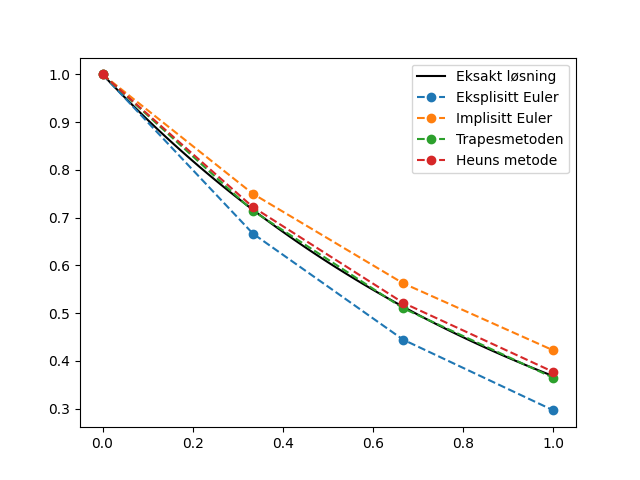
\includegraphics[scale=0.6]{methods_test.png}
    \end{center}

    Nå kan vi endre på steglengden $h$ for å undersøke hvor godt metodene fungerer.

\end{ex}



\end{document}
